\documentclass{article}

\usepackage{graphicx}
\usepackage{tikz}
\usepackage{tikzsymbols}
\usetikzlibrary{calc,patterns,shapes.geometric}
\pagestyle{empty}
\usepackage[margin=0pt]{geometry}
\geometry{papersize={14in,12in}}

\def\centerarc[#1](#2)(#3:#4:#5){\draw[#1] ($(#2)+({#5*cos(#3)},{#5*sin(#3)})$) arc (#3:#4:#5);}

\begin{document}
	\begin{figure}
		\centering
		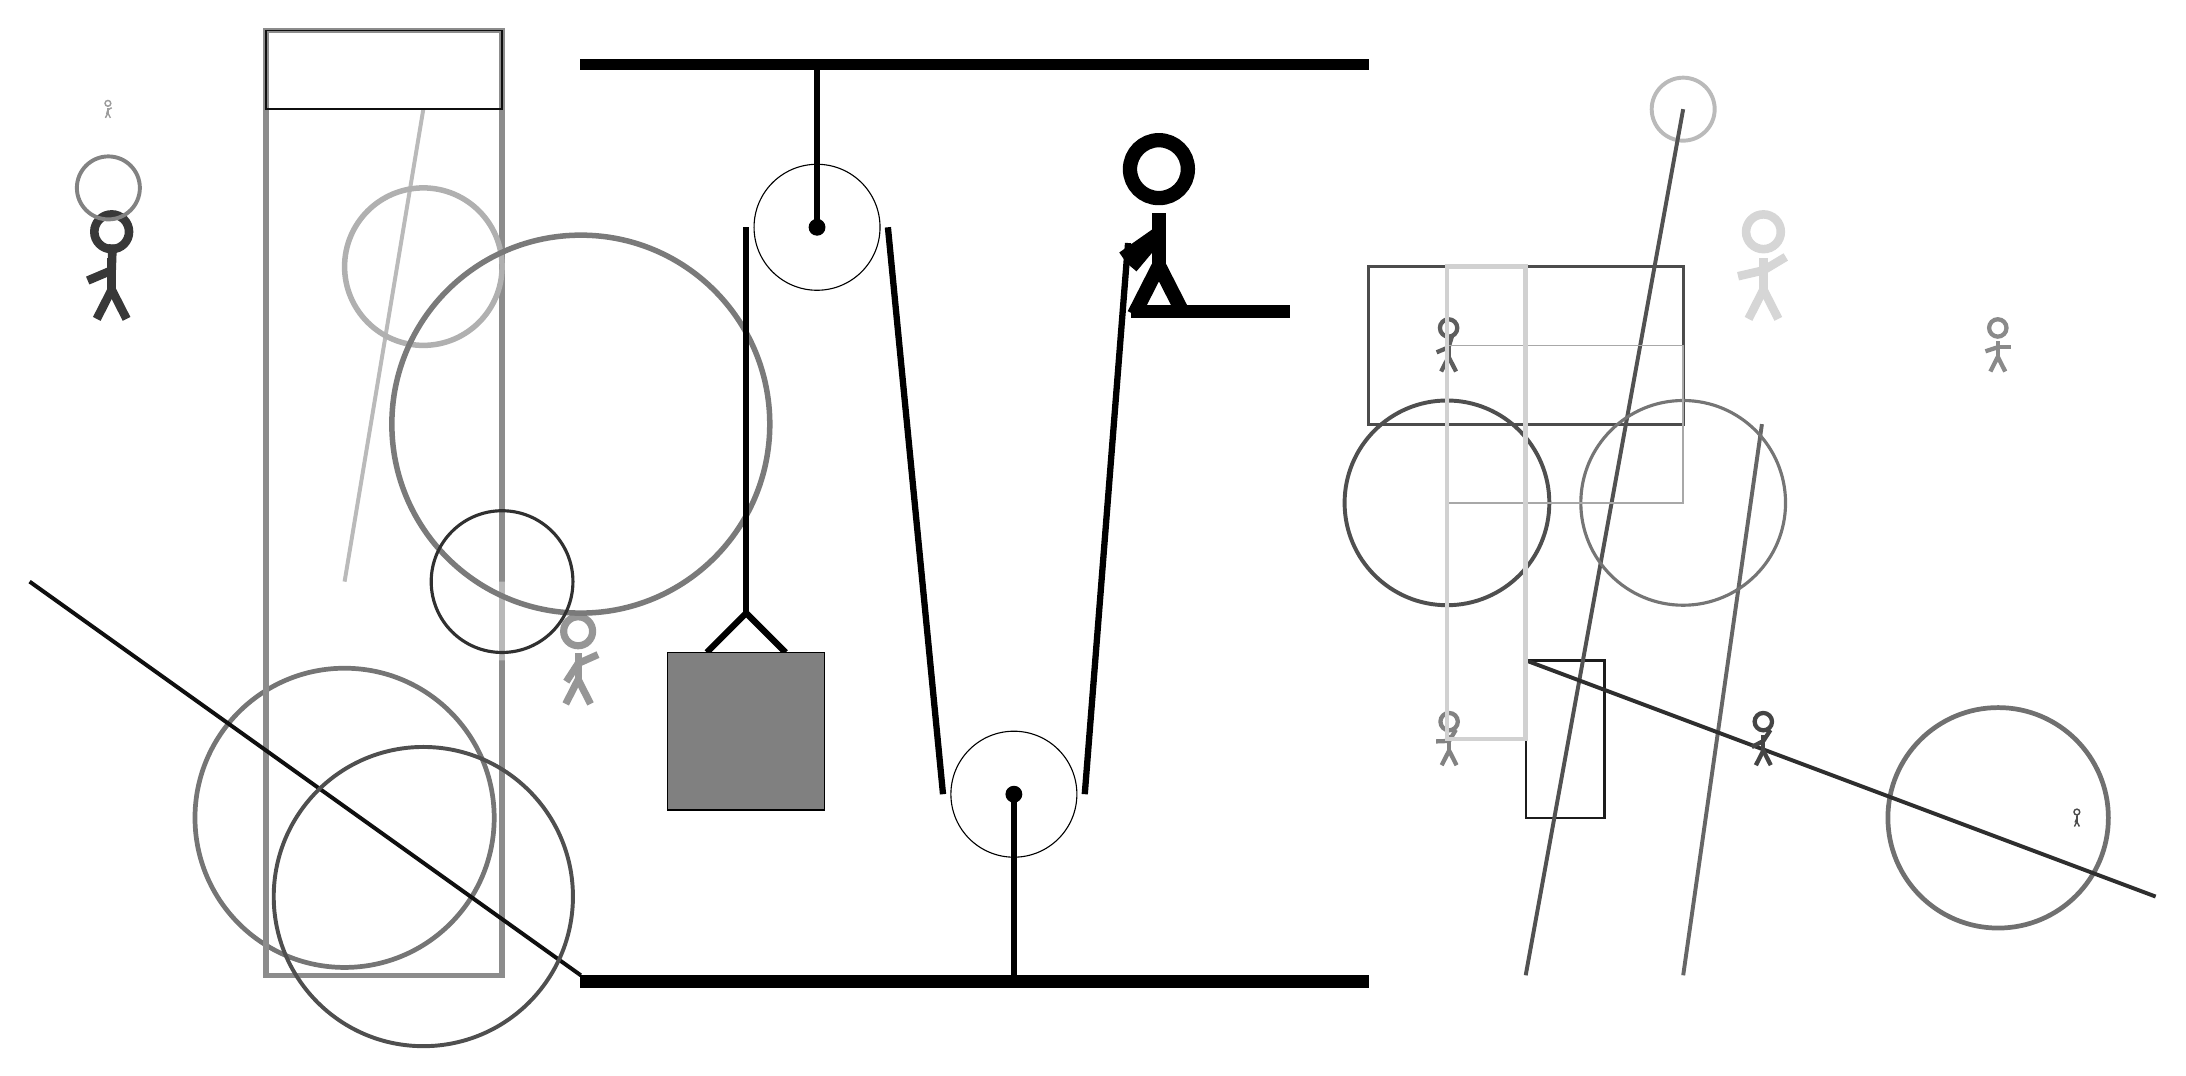
\begin{tikzpicture}
			%%%%% START %%%%%
			
			\draw[fill=black] (-2, 11.5) rectangle (8, 11.625);
			
			\draw[line width=0.3mm, color=black!89] (10, 4) rectangle (11, 2);
			
			\draw [line width=0.6mm, color=black!54](-5, 2) circle (1.9);
			\draw [line width=0.5mm, color=black!27](12, 11) circle (0.4);
			\node[line width=0.7mm, color=black!78] at (-8, 9) {\Strichmaxerl[6][23][88]};
			
			\draw[line width=0.7mm, color=black!45] (-3, 12) rectangle (-6, 0);
			\draw[line width=0.4mm, color=black!70] (8, 7) rectangle (12, 9);
			\node[line width=0.7mm, color=black!70] at (17, 2) {\Strichmaxerl[1][66][83]};
			
			\draw[line width=0.5mm, color=black!27](-5, 5) -- (-4, 11);
			\draw[line width=0.5mm, color=black!68](12, 11) -- (10, 0);
			\draw[line width=0.5mm, color=black!60](13, 7) -- (12, 0);
			\node[line width=0.2mm, color=black!16] at (13, 9) {\Strichmaxerl[6][13][31]};
			\draw[line width=0.7mm, color=black!28] (-3, 4) rectangle (-3, 5);
			\node[line width=0.2mm, color=black!63] at (9, 8) {\Strichmaxerl[3][23][73]};
			
			\draw [line width=0.7mm, color=black!31](-4, 9) circle (1.0);
			\draw[line width=0.5mm, color=black!94](-2, 0) -- (-9, 5);
			\draw [line width=0.4mm, color=black!54](12, 6) circle (1.3);
			\node[line width=0.3mm, color=black!46] at (16, 8) {\Strichmaxerl[3][18][0]};
			\draw [line width=0.5mm, color=black!69](-4, 1) circle (1.9);
			\draw [line width=0.6mm, color=black!56](16, 2) circle (1.4);
			\node[line width=0.4mm, color=black!49] at (9, 3) {\Strichmaxerl[3][2][59]};
			\node[line width=0.2mm, color=black!41] at (-2, 4) {\Strichmaxerl[5][57][24]};
			
			\draw [line width=0.7mm, color=black!52](-2, 7) circle (2.4);
			
			\draw [line width=0.4mm, color=black!81](-3, 5) circle (0.9);
			\draw[line width=0.5mm, color=black!82](10, 4) -- (18, 1);
			\draw [line width=0.5mm, color=black!69](9, 6) circle (1.3);
			\draw[line width=0.2mm, color=black!34] (9, 8) rectangle (12, 6);
			\node[line width=0.2mm, color=black!73] at (13, 3) {\Strichmaxerl[3][28][57]};
			\node[line width=0.7mm, color=black!39] at (-8, 11) {\Strichmaxerl[1][73][28]};
			\draw[line width=0.2mm, color=black!94] (-3, 12) rectangle (-6, 11);
			\draw[line width=0.7mm, color=black!50] (9, 4) rectangle (9, 4);
			\draw [line width=0.5mm, color=black!49](-8, 10) circle (0.4);
			
			\draw[line width=0.6mm, color=black!18] (9, 3) rectangle (10, 9);
			
			\draw (3.5, 2.3) circle (0.8);
			\draw[fill=black] (3.5, 2.3) circle (0.1);
			\draw[line width=0.8mm] (3.5, 2.3) -- (3.5, 0);
			
			\draw (1, 9.5) circle (0.8);
			\draw[fill=black] (1, 9.5) circle (0.1);
			\draw[line width=0.8mm] (1, 11.5) -- (1, 9.5);
			
			\draw[line width=0.8mm](-0.4, 4.1) --  (0.1, 4.6) -- (0.6, 4.1);
			\draw[fill=black!50] (-0.9, 4.1) rectangle (1.1, 2.1);
			
			\draw[line width=0.8mm](0.1, 9.5) -- (0.1, 4.6);
			\centerarc[line width=0.8mm](1, 9.5)(180:0:0.9)
			\draw[line width=0.8mm](1.9, 9.5) -- (2.6, 2.3);
			\centerarc[line width=0.8mm](3.5, 2.3)(180:360:0.9)
			\draw[line width=0.8mm](4.4, 2.3) -- (4.95, 9.3);
			
			\node at (5.3, 9.5) {\Strichmaxerl[10][35][-130]};
			\draw[fill=black] (5, 8.5) rectangle (7, 8.35);
			
			\draw[fill=black] (-2, 0) rectangle (8, -0.15);
			
			%%%%% END %%%%%
		\end{tikzpicture}
	\end{figure}	
\end{document}